% !TeX spellcheck = en_GB
%%%%%%%%%%%%%%%%%%%%%%%%%%%%%%%%%%%%%%%%%%%%%%%%%%%%%%%%%%%%%%%%%%%%%%%%%%%%%%%%
% SD Lab -- Build Automation
% Giovanni Ciatto
% Alma Mater Studiorum - Università di Bologna
% mailto:giovanni.ciatto@unibo.it
%%%%%%%%%%%%%%%%%%%%%%%%%%%%%%%%%%%%%%%%%%%%%%%%%%%%%%%%%%%%%%%%%%%%%%%%%%%%%%%%
%\documentclass[handout]{beamer}\mode<handout>{\usetheme{default}}
%
\documentclass[presentation]{beamer}\mode<presentation>{\usetheme{AMSBolognaFC}}
%\documentclass[handout]{beamer}\mode<handout>{\usetheme{AMSBolognaFC}}
%%%%%%%%%%%%%%%%%%%%%%%%%%%%%%%%%%%%%%%%%%%%%%%%%%%%%%%%%%%%%%%%%%%%%%%%%%%%%%%%
\usepackage{sd-lab-common}
\usepackage{sd-lab-automation}
%%%%%%%%%%%%%%%%%%%%%%%%%%%%%%%%%%%%%%%%%%%%%%%%%%%%%%%%%%%%%%%%%%%%%%%%%%%%%%%%
\title[\currentLab{} -- Build Automation]{
	Build Automation 101
}
%
\subtitle{\courseName{} (\courseAcronym) / Module \moduleN{}}
%
\author[\sspeaker{\gcShort} \& \mmShort]{
	\speaker{\gcFull} \and \mmFull
	\\
	\gcEmail \and \mmEmail
}
%
\institute[\disiShort, \uniboShort]{\disi{} (\disiShort)\\\unibo}
%
\date[A.Y. \academicYear{}]{Academic Year \academicYear{}}
%
\begin{document}

\maketitle

\begin{frame}[c]\frametitle{Outline}
    % \begin{multicols}{2}
	    \tableofcontents[sectionstyle=show/show, subsectionstyle=show/show, subsubsectionstyle=show/show]
    % \end{multicols}
\end{frame}

\section{Motivation}

\begin{frame}[allowframebreaks]
\frametitle{Motivation}

    \begin{itemize}
        \item Real world (distributed) applications are made up of several \alert{components} which need to be \alert{deployed} on one or more machines
        %
        \begin{itemize}
            \item possibly in an orderly fashion
        \end{itemize}

        \bigskip

        \item Furthermore, only rarely people write software \alert{from scratch}
        %
        \begin{itemize}
            \item more commonly, software \alert{depends} from other software
            %
            \begin{itemize}
                \item which may depend on further software, and so on
            \end{itemize}

            \item[$\rightarrow$] dependencies cannot be \alert{manually} handled
            %
            \begin{itemize}
                \item error prone, time consuming task
            \end{itemize}
        \end{itemize}

        \framebreak

        \item In projects/exercises, you may need to write, compile, \alert{deploy}, \& start several processes in a given \alert{order}, possibly multiple \alert{times}
        %
        \begin{itemize}
            \item furthermore we may will to exploit \alert{open-source libraries} from the Internet
        \end{itemize}

        \bigskip


        \item We will extensively leverage \alert{Build Automation} in our activities to automate most low level operations
        %
        \begin{itemize}
            \item in an IDE-independent way
            \item (activities include exercises and final projects :)
        \end{itemize}

    \end{itemize}

\end{frame}

% \begin{frame}
% \frametitle{Lecture goals II}

%     \begin{itemize}
%         \item<1> In this course, you may need a way to reproduce Lab exercises on your personal computers, possibly simulating a distributed environment

%         \vfill{}

%         \item<2> Furthermore, you must be able to submit your homeworks/projects being sure they will run on other computer too
%         \begin{itemize}
%             \item<2> Avoiding the situation \emph{``No, I swear, it used to work on my PC''} :)

%             \item<2>[!] Making your results more durable and \alert{reproducible}
%         \end{itemize}

%         \vfill{}

%         \item<3>[$\rightarrow$] You will learn some fundamentals of:
%         \begin{itemize}
%             \item<3> Build \& automation systems (e.g. \href{https://gradle.org/}{Gradle})
%             \item<3> Container Engines (e.g. \href{https://www.docker.com/}{Docker})
%         \end{itemize}

%         \vfill{}

%         \item<4> Because of Lab-0, you are assumed to:
%         \begin{itemize}
%             \item<4> have properly installed Gradle and Docker on your personal PC
%             \item<4> have a Docker ID with your \texttt{@studio.unibo.it} email address
%         \end{itemize}
%     \end{itemize}

% \end{frame}

\section{Build Automation Systems}

\subsection{Overview}

\begin{frame}{Build Automation Systems}
    Build automation systems \alert{automate} several sub-tasks of the SW developing \& engineering process, like for instance:
    %
    \begin{multicols}{2}
        \begin{itemize}
            \item Dependencies management

            \item \alert{Compilation}

            \item Code generation

            \item Testing

            \item Execution

            \item Artefact generation
            %
            \begin{itemize}
                \item[eg] \texttt{.jar} files
            \end{itemize}

            \item Release publication/upload
        \end{itemize}
    \end{multicols}
    %
    just to cite some.

    \vfill

    \begin{itemize}

        \item Remember the time spent configuring someone else's Eclipse project?
        %
        \begin{itemize}
            \item we are targeting that problem
        \end{itemize}

        \item[!] Plus, build automation systems are very handy when combined with Containers, e.g. for Continuous Integration

    \end{itemize}


\end{frame}

\subsection{Gradle}

\begin{frame}{Build Automation systems for the JVM}
    We will leverage \alert{Gradle} as a build automation system for JVM-based application in order to automate your exercises/projects:
    %
    \begin{itemize}
        \item dependencies management
        \item compilation
        \item launch by command line
    \end{itemize}

    \vfill

    (Of course, alternatives exist for other platforms)

    \vfill

    \begin{block}{From now on}
        \begin{itemize}
            \item JVM projects \emph{should} be submitted as self-contained Gradle projects
        \end{itemize}
    \end{block}
\end{frame}

\begin{frame}{Build Automation systems for other platforms}

    \begin{table}[H!]
        \centering
        \begin{tabular}{c|c|c}
            \textbf{Platform} & \textbf{Build Automation System} & \textbf{Package Repository}
            \\\hline\hline
            JVM               & Gradle / Maven                   & \href{https://search.maven.org/}{MCR}
            \\
            Python            & pip + setuptools + virtualenv\footnotemark    & \href{https://pypi.org/}{Pypi}
            \\
            .NET              & dotnet                           & \href{https://www.nuget.org/}{NuGet}
            \\
            JavaScript        & npm                              & \href{https://www.npmjs.com/}{NPM}
        \end{tabular}
    \end{table}

    \footnotetext{cf. \uurl{https://stackoverflow.com/questions/41573587/what-is-the-difference-between-venv-pyvenv-pyenv-virtualenv-virtualenvwrappe}}

    \vfill

    \begin{block}{From now on}
        \begin{itemize}
            \item projects targetting platform $X$ \emph{should} be submitted with the most adequate build automation facilities for platform $X$
        \end{itemize}
    \end{block}
\end{frame}

\begin{frame}[allowframebreaks]
\frametitle{Gradle in a Nutshell}

    Gradle is our build automation of choice
    %
    \bigskip
    %
    \begin{itemize}
        \item It assumes each project to adhere to a well defined \alert{directory structure}
        %
        \begin{itemize}
            \item possibly involving several \alert{sub-projects} (a.k.a. \alert{modules})\ldots
            \item \ldots in this case we distinguish among the \alert{root} project and many \alert{sub-}projects
            %
            \begin{itemize}
                \item we may refer to both as \emph{projects}, in general
            \end{itemize}
        \end{itemize}

        \bigskip

        \item Projects and sub-projects are \alert{computational units}
        %
        \begin{itemize}
            \item[ie] containers of code which are compiled, tested, and packed \alert{as wholes}
            \item it is quite common for (sub-)projects to be \alert{inter-dependent}
        \end{itemize}

        \framebreak

        \item The \alert{root} project is special, as its directory contains:
        %
        \begin{itemize}
            \item a \alert{\texttt{gradlew}} script (\texttt{gradlew.bat}, on Windows systems)
            %
            \begin{itemize}
                \item it is called the \alert{Gradle wrapper}
                \item it's your entry point manage either root project or any sub-projects
            \end{itemize}

            \item a \alert{\texttt{settings.gradle(.kts)}} script
            %
            \begin{itemize}
                \item declaring the root project's and sub-projects' names
            \end{itemize}
        \end{itemize}

        \bigskip

        \item Each project should contain a \alert{\texttt{build.gradle(.kts)}} file
        %
        \begin{itemize}
            \item either explicitly or implicitly declaring the \alert{properties} of that project
            %
            \begin{itemize}
                \item[eg] language, SDK, dependencies, compilation options, metadata, etc
            \end{itemize}

            \item either explicitly or implicitly defining \alert{tasks} of that project
            %
            \begin{itemize}
                \item[eg] build, test, assemble, etc., and their
            \end{itemize}
        \end{itemize}

        \framebreak

        \item Notably, dependencies are just \alert{declared} into a \alert{\texttt{build.gradle(.kts)}} file, along with their versions
        %
        \begin{itemize}
            \item no \texttt{.jar} file must/should be provided, in the general case
            \item retrieval is automatic, from a number of \alert{package repositories}
            %
            \begin{itemize}
                \item[eg] the \href{https://search.maven.org/}{Maven Central Repository (MCR)} repository
            \end{itemize}
            \item package repositories URL must be declared as well!
        \end{itemize}

        \bigskip

        \item Each project's source code is stored into the \alert{\texttt{src}} directory, and partitioned\ldots
        %
        \begin{itemize}
            \item \ldots by source set (commonly, \alert{\texttt{main}} and \alert{\texttt{test}})
            %
            \begin{itemize}
                \item \ldots and by language (commonly, \alert{\texttt{java}}, \texttt{kotlin}, \texttt{scala}, etc.)
                \item[!] \alert{\texttt{resources}} are considered as yet another sort of language
            \end{itemize}
            \item main code is packed and deployed, test code is not
        \end{itemize}

        \framebreak

        \item Under such hypotheses, developers can execute several tasks on the project by calling the \texttt{gradlew} script as follows:
        %
        \begin{itemize}
            \item[\$] \texttt{\alert{./}gradlew \alert{<task>}} \quad (on Unix)
            \item[] or
            \item[$>$] \texttt{\alert{.$\backslash$}gradlew \alert{<task>}} \quad (on Windows)
            %
            \begin{itemize}
                \item[!] we will only write the Unix syntax henceforth
            \end{itemize}
        \end{itemize}

        \bigskip

        \item If Gradle is properly installed on your system, you don't need the \texttt{gradlew} script:
        %
        \begin{itemize}
            \item[\$] \texttt{gradle \alert{<task>}} \quad (on both Unix and Windows)
            %
            \begin{itemize}
                \item[!] prefer using the wrapper when available
            \end{itemize}
        \end{itemize}

        \bigskip

        \item A sub-project's specific task can be launched by:
        %
        \begin{itemize}
            \item[\$] \texttt{./gradlew \alert{<sub-project>}:\alert{<task>}}
        \end{itemize}

        \framebreak

        \item The set of available tasks (for JVM apps) includes:
        %
        \begin{description}
            \item[\texttt{assemble}] --- compiles the projects
            \item[\texttt{check}] --- runs the user-defined tests
            \item[\texttt{build}] --- compiles the project \& runs the tests
            \item[\texttt{run}] --- runs the application
            \item[\texttt{tasks}] --- shows a list of available tasks
        \end{description}

        \bigskip

        \item Dependencies between are as follows:
        %
        \begin{itemize}
            \item \texttt{run} $\rightarrow$ \texttt{build} $\rightarrow$ \texttt{check} $\rightarrow$ \texttt{assemble}

            \item so if you try to run an unassembled application, it will be
            %
            \begin{itemize}
                \item firstly \alert{assembled} (i.e., compiled)
                \item then \alert{checked} (i.e., tested)
                \item and finally \alert{run}
            \end{itemize}
        \end{itemize}
    \end{itemize}

\end{frame}

\subsubsection{Canonical Directory Structures}

\begin{frame}[fragile]
\frametitle{Canonical Directory Structure -- Flat Project}

\begin{Verbatim}[fontsize=\small,commandchars=\\\{\}]
\textcolor{blue}{my-project/}\dhint{The root project directory, named after it}
├── \textcolor{green}{gradlew}\dhint{The \emph{Gradle Wrapper} script, for Unix}
├── \textcolor{green}{gradlew.bat}\dhint{The \emph{Gradle Wrapper} script, for Windows}
├── \textcolor{olive}{build.gradle[.kts]}\dhint{Project configuration of the project}
├─┬ \textcolor{cyan}{src/}\dhint{The \emph{source} folder: contains the project code}
│ ├─┬ main/\dhint{The 'main' \emph{source set}, contains the application code}
│ │ └─┬── java/\dhint{Java source files}
│ │   ├?─ kotlin/\dhint{Kotlin source files}
│ │   └?─ \textcolor{orange}{resources/}\dhint{The application resource files}
│ └?┬ test/\dhint{The 'test' \emph{source set}, contains the tests code}
│   └─┬?─ <other lang>/
│     └?─ \textcolor{orange}{resources/}
├?─ \textcolor{gold}{gradle.properties}\dhint{A \href{https://en.wikipedia.org/wiki/.properties}{\emph{.properties} file} for default properties}
├?─ \textcolor{olive}{settings.gradle[.kts]}\dhint{Name of the root project and of all \emph{sub-projects}}
├── \textcolor{red}{gradle/}\dhint{Contains libraries for the Gradle Wrapper}
├── \textcolor{red}{.gradle/}\dhint{Dynamically generated by the Gradle Wrapper}
└── \textcolor{red}{build/}\dhint{Where compiled \emph{.class} and \emph{.jar} files are put}
\end{Verbatim}

\end{frame}

\begin{frame}[fragile]
    \frametitle{Canonical Directory Structure -- Multi-Project}

\begin{Verbatim}[fontsize=\tiny,commandchars=\\\{\}]
\textcolor{blue}{my-project/}\dhint{The \emph{root project} directory, named after it}
├── \textcolor{green}{gradlew}\dhint{The \emph{Gradle Wrapper} script, for Unix}
├── \textcolor{green}{gradlew.bat}\dhint{The \emph{Gradle Wrapper} script, for Windows}
├── \textcolor{olive}{build.gradle[.kts]}\dhint{Configuration of the \emph{root project}}
├?┬ \textcolor{cyan}{src/}\dhint{The \emph{source} folder: contains the \emph{root project}'s code}
│  ├─┬ main/\dhint{The `main' \emph{source set} of the \emph{root project}}
│  │  └─┬── java/\dhint{Java source files of the \emph{root project}}
│  │      ├?─ kotlin/\dhint{Kotlin source files of the \emph{root project}}
│  │      └?─ \textcolor{orange}{resources/}\dhint{Resource files for the \emph{root project}}
│  └?┬ test/\dhint{The `test' \emph{source set} of the \emph{root project}}
│     └─┬?─ <other lang>/
│         └?─ \textcolor{orange}{resources/}
├─┬ \textcolor{blue}{sub-project-1/}\dhint{Root of the \emph{sub-project-1}}
│  ├── \textcolor{olive}{build.gradle[.kts]}\dhint{Configuration of \emph{sub-project-1}}
│  ├─┬ \textcolor{cyan}{src/}\dhint{\emph{Source} folder of \emph{sub-project-1}}
│  │  └── \ldots
│  └?─ \textcolor{gold}{gradle.properties}\dhint{A \href{https://en.wikipedia.org/wiki/.properties}{\emph{.properties} file} for default properties of \emph{sub-project-1}}
├─┬ \textcolor{blue}{sub-project-2/}\dhint{Root of the \emph{sub-project-2}}
│  ├── \textcolor{olive}{build.gradle[.kts]}\dhint{Configuration of \emph{sub-project-2}}
│  ├─┬ \textcolor{cyan}{src/}\dhint{\emph{Source} folder of \emph{sub-project-2}}
│  │  └── \ldots
│  └?─ \textcolor{gold}{gradle.properties}\dhint{A \href{https://en.wikipedia.org/wiki/.properties}{\emph{.properties} file} for default properties of \emph{sub-project-2}}
├?─ \textcolor{gold}{gradle.properties}\dhint{A \href{https://en.wikipedia.org/wiki/.properties}{\emph{.properties} file} for default properties}
├── \textcolor{olive}{settings.gradle[.kts]}\dhint{Some minor project settings, in Gradle lang}
├── \textcolor{red}{gradle/}\dhint{Contains libraries for the Gradle Wrapper}
├── \textcolor{red}{.gradle/}\dhint{Dynamically generated by the Gradle Wrapper}
└── \textcolor{red}{build/}\dhint{Where compiled \emph{.class} and \emph{.jar} files are put}
\end{Verbatim}
\end{frame}

\begin{frame}[allowframebreaks]
\frametitle{Gradle Files}

\begin{block}{Gradle files you may need to read/edit}
    \begin{description}
        \item[\texttt{settings.gradle}] $\rightarrow$ Groovy syntax
        %
        \begin{itemize}
            \item Kotlin syntax $\rightarrow$ add the \alert{\texttt{.kts}} extension
        \end{itemize}

        \item[\texttt{build.gradle}] $\rightarrow$ Groovy syntax
        %
        \begin{itemize}
            \item Kotlin syntax $\rightarrow$ add the \alert{\texttt{.kts}} extension
        \end{itemize}

        \item[\texttt{gradle.properties}] $\rightarrow$ Java's \texttt{.properties}\footnote{cf. \url{https://en.wikipedia.org/wiki/.properties}} syntax
        %
        \begin{itemize}
            \item essentially, \texttt{\textit{key}\alert{=}value} entries, one per line
        \end{itemize}
    \end{description}
\end{block}
%
\begin{itemize}
    \item[!] we suggest using the Kotlin syntax
\end{itemize}

\lstinputlisting[
    basicstyle=\ttfamily\scriptsize,
    language=Kotlin,
    caption={General structure of \texttt{settings.gradle.kts}},
    captionpos=b
]{src/settings.gradle.kts}

\framebreak

\lstinputlisting[
basicstyle=\ttfamily\tiny,
language=Kotlin,
caption={General structure of \texttt{build.gradle.kts}},
captionpos=b
]{src/pattern-of-build.gradle.kts}

\framebreak

\lstinputlisting[
basicstyle=\ttfamily\tiny,
language=Kotlin,
caption={Example of \texttt{build.gradle.kts}},
captionpos=t
]{src/build.gradle.kts}

\end{frame}

\begin{frame}[allowframebreaks]
    \frametitle{Handling dependencies}

    Dependencies -- i.e., specific versions of artefacts -- can be added by appending to the \texttt{dependencies} section lines of the form
    %
    \begin{center}
        \texttt{implementation\textit{<Scope>}("\textit{<gropuId>}\alert{:}\textit{<artifactId>}\alert{:}\textit{<version>"}})
    \end{center}
    %
    \begin{description}\small
        \item[\texttt{gropuId}] identifies a group of related artefacts
        \item[\texttt{artifactId}] identifies a specific artefact within the group
        \item[\texttt{version}] identifies a specific version of that artefact
        \item[\texttt{Scope}] is \alert{\texttt{Test}} for test dependencies, or the empty string otherwise
    \end{description}

    \medskip

    BTW, versions are usually expressed through Semantic Versioning \ccite{semVer}
    %
    \begin{center}
        \texttt{"\textit{<MAJOR>}\alert{.}\textit{<MINOR>}\alert{.}\textit{<PATCH>"}}
    \end{center}
    %
    \begin{description}\small
        \item[\texttt{MAJOR}] increases when non-retro-compatible changes are done
        \item[\texttt{MINOR}] increases when retro-compatible changes are done
        \item[\texttt{PATCH}] increases when implementation details are changed
    \end{description}

    \framebreak

    Artefacts -- along with their \texttt{groupId}, \texttt{artifactID} and \texttt{version} -- are hosted on repositories such as \href{https://search.maven.org/}{Maven Central} or \href{https://bintray.com/bintray/jcenter}{JCenter} (deprecated)
    %
    \begin{center}
        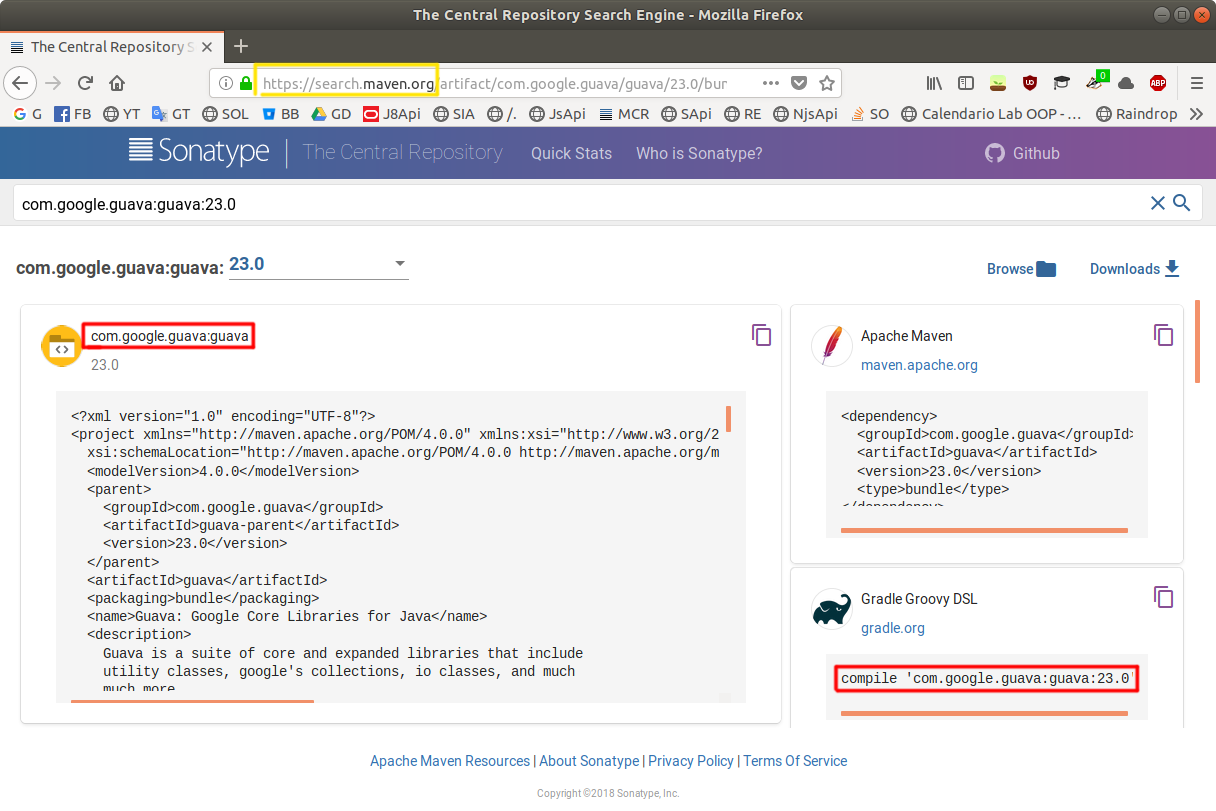
\includegraphics[width=.6\linewidth]{./img/mcr.png}

        {\scriptsize\url{https://search.maven.org/artifact/com.google.guava/guava/30.1.1-jre/bundle}}
    \end{center}

\end{frame}

\subsection{Authoring Tasks}

\begin{frame}[allowframebreaks]
\frametitle{Editing an existing task}
    \lstinputlisting[
        language=Kotlin,
        caption={General way of editing a default task},
        captionpos=b
    ]{src/edit-default-tasks.kt}

    \lstinputlisting[
        language=Kotlin,
        caption={Example: editing the \texttt{test} and \texttt{compileJava} tasks},
        captionpos=b
    ]{src/edit-default-tasks-example.kt}

    \framebreak

    \lstinputlisting[
        language=Kotlin,
        caption={General way of editing any task},
        captionpos=b
    ]{src/edit-custom-tasks.kt}

    \lstinputlisting[
        basicstyle=\ttfamily\tiny,
        language=Kotlin,
        caption={General way of editing any task},
        captionpos=b
    ]{src/edit-custom-tasks-example.kt}

\end{frame}

\begin{frame}[allowframebreaks]
    \frametitle{Creating a new task}
    \lstinputlisting[
        language=Kotlin,
        caption={General way of creating a custom task},
        captionpos=t
    ]{src/create-custom-tasks.kt}

    \begin{block}{About groups and descriptions}
        \begin{itemize}
            \item The are basic properties following documentations purposes
            \item They aid developers willing to explore tasks via:
            %
            \begin{itemize}
                \item[\$] \texttt{./gradle tasks}
            \end{itemize}
        \end{itemize}
    \end{block}

    \framebreak

    \lstinputlisting[
        basicstyle=\ttfamily\tiny,
        language=Kotlin,
        caption={Example 1: creating a \texttt{JavaExec} task},
        captionpos=b
    ]{src/my-custom-java-exec-task.kt}

    \framebreak

    \lstinputlisting[
        basicstyle=\ttfamily\tiny,
        language=Kotlin,
        caption={Example 2: creating an \texttt{Exec} task},
        captionpos=b
    ]{src/my-custom-exec-task.kt}

\end{frame}

\begin{frame}[allowframebreaks]
\frametitle{Passing arguments to Gradle tasks}

    \begin{itemize}
        \item Gradle tasks accept arguments in the form of \alert{properties}
        \item A property is a \alert{key-value} pair
        \item The behaviour of tasks can be parametrised via properties
    \end{itemize}

    \framebreak

    \lstinputlisting[
        basicstyle=\ttfamily\tiny,
        language=Kotlin,
        caption={General way of reading a property in a Gradle script},
        captionpos=b
    ]{src/consuming-properties.kt}

    \framebreak

    Three ways to ``pass'' a property to Gradle:

    \begin{block}{Pass key-value pairs by command line to \texttt{gradlew}}
        \centering
        \alert{\$} \texttt{./gradlew \textit{<task>} -P}\alert{\texttt{key1}}\texttt{=}\alert{\texttt{value1}} \texttt{-P}\alert{\texttt{key2}}\texttt{=}\alert{\texttt{value2}} \texttt{...}
    \end{block}

    \begin{block}{Append lines a \texttt{gradle.properties} file}
        \alert{\texttt{key1}}\texttt{=}\alert{\texttt{value1}}\\
        \alert{\texttt{key2}}\texttt{=}\alert{\texttt{value2}}\\
        \texttt{...}
    \end{block}

    \begin{block}{Define an environment variable with a particular name}
        \centering
        \alert{\$} \texttt{\textit{export} ORG\_GRADLE\_PROJECT\_\alert{key}=\alert{value}}
        %
        \begin{itemize}
            \item[!] before launching \texttt{gradle} or \texttt{gradlew}
        \end{itemize}
    \end{block}

    \framebreak

    \lstinputlisting[
        basicstyle=\ttfamily\tiny,
        language=Kotlin,
        caption={Example of reading custom properties in a Gradle script},
        captionpos=b
    ]{src/run.task.kts}

\end{frame}

\subsection{Running Gradle}

\begin{frame}
    \framebreak{About running Gradle}

    \begin{block}{Gradle daemon}
        \begin{itemize}
            \item The first time Gradle is launched it starts a daemon
            %
            \begin{itemize}
                \item to speed subsequent runs up
            \end{itemize}
            \item The daemon may survive the single run
            %
            \begin{itemize}
                \item provoking issues in some cases
            \end{itemize}
            \item To prevent that, use the \alert{\texttt{{-}-no-daemon}} argument
        \end{itemize}
    \end{block}

    \begin{block}{Gradle logs}
        \begin{itemize}
            \item Gradle logs a number of useful information\ldots
            \item \ldots and erases most of them on the fly
            \item Use the \alert{\texttt{{-}-console=plain}} argument to avoid erasure
            \item Use the \alert{\texttt{-q}} argument to avoid logs
        \end{itemize}
    \end{block}
\end{frame}

\subsection{Importing Gradle Projects into IDE}

\begin{frame}[c,allowframebreaks]
	\frametitle{How to import Gradle Projects into Eclipse}

	\begin{block}{\textbf{Takeway} -- Preferred setup for Eclipse}
		\begin{itemize}
			\item Put your Gradle root project inside a directory, inside the \alert{workspace}
			\item[eg] \texttt{/path/to/workspace}
			%
			\begin{itemize}
				\item[] \texttt{/path/to/workspace/\alert{my-app}}
				%
				\begin{itemize}
					\item[] \texttt{/path/to/workspace/my-app/\alert{build.gradle.kts}}
				\end{itemize}
			\end{itemize}
		\end{itemize}
	\end{block}

	\framebreak

	\begin{enumerate}
		\item Move directory \texttt{/path/to/\alert{my-app}} to \texttt{/path/to/\alert{workspace}/my-app}
        %
        \begin{itemize}
            \item or use \texttt{/path/\alert{to/}} as the workspace
        \end{itemize}

		\medskip

		\item Open Eclipse, choosing \texttt{/path/to/\alert{workspace}} as workspace

		\medskip

		\item Click on $File$ and then select $Import$: a wizard should appear
		%
		\begin{enumerate}
			\item select $Gradle / Exsting\ Gradle\ Project$
			\item click on $Next$ as may times as possible
			\item click on $Finish$
		\end{enumerate}

		\medskip

		\item The Gradle project should now be correctly imported
		%
		\begin{itemize}
			\item its dependencies should be automatically loaded
		\end{itemize}

		\medskip

		\item Use Eclipse as usual

		\medskip

		\item Notice the $Gradle\ Tasks$ view letting you launch tasks from the GUI

	\end{enumerate}

\end{frame}

\startExercise

\begin{frame}%[c,allowframebreaks]
	\frametitle{Import Gradle Projects into IntelliJ Idea}

	\begin{enumerate}
		\item From the welcome page: click on $Open\ or\ Import$
		%
		\begin{itemize}
			\item equivalently, from an open Idea Window: $File > Open\ldots$
		\end{itemize}

		\medskip

		\item Select (or just write) the path of your root project, then press $Ok$
		%
		\begin{itemize}
			\item[ie] \texttt{/path/to/\alert{my-app}}
			\item refresh if you cannot find a directory that should be there
		\end{itemize}

		\medskip

		\item If prompted, import the project as a Gradle project
		%
		\begin{itemize}
			\item \emph{not} an Eclipse one
		\end{itemize}

		\medskip

		\item The Gradle project should now be correctly imported
		%
		\begin{itemize}
			\item its dependencies should be automatically loaded
		\end{itemize}

		\medskip

		\item Use IntelliJ Idea as usual

		\medskip

		\item Notice the $Gradle$ view letting you launch tasks from the GUI

	\end{enumerate}

\end{frame}

\section{Exercises}

\subsection{Gradlefying JVM Projects}

\startExercise

\begin{frame}[allowframebreaks]
	\frametitle{Exercise \currentExercise{} -- Gradlefying a JVM project}

	\begin{block}{Repository}\centering
		\url{\gitlabGroup/lab-1}
	\end{block}

	\bigskip

	Activity:
	%
	\medskip
	%
	\begin{enumerate}
		\item Have a look to the provided code: it contains the \alert{JEcho} application
		%
		\begin{itemize}
			\item aimed at echoing the standard input using one of \alert{three modalities}
			%
			\begin{itemize}
				\item upper/lower case, or just normal
			\end{itemize}
			\item using an external dependency, via local \texttt{.jar} files
			%
			\begin{itemize}
				\item namely, \href{https://commons.apache.org/proper/commons-cli/}{Apache's Commons CLI} tools
			\end{itemize}
		\end{itemize}

		\medskip

		\item Inspect and understand the code

		\framebreak

		\item Gradlefy the project
		%
		\begin{itemize}
			\item generate the \texttt{gradlew(.bat)}, \texttt{build.gradle.kts}, etc. files
			\item adopt Gradle's canonical directory structure
			\item delete the \texttt{.jar} dependencies, and declare them instead
		\end{itemize}

		\medskip

		\item Set up Gradle's \texttt{run} task to launch JEcho
		%
		\begin{itemize}
			\item use an optional property named \texttt{`mode'} to let users specify the working modality of JEcho
			\item \texttt{`lowercase'} or \texttt{`uppercase'} are the admissible values for \texttt{mode}
		\end{itemize}

		\medskip

		\item[!] Solutions which do not pass the tests are not correct
		%
		\begin{itemize}
			\item tests are provided as Bash scripts, for *nix systems
		\end{itemize}

		\medskip

		\item Push your solution on GitLab, \alert{even if incomplete}
		%
		\begin{itemize}
			\item use the \texttt{submissions/\alert{name.surnameN}} branch
			\item tests are automatically run upon push: consider it a feedback
		\end{itemize}

	\end{enumerate}

\end{frame}

%===============================================================================
\section*{}
%===============================================================================
\frame{\titlepage}

%===============================================================================
\section*{\bibname}
%===============================================================================

\setbeamertemplate{page number in head/foot}{}
%\\\\\\\\\\\\\\\\\\\\\
\begin{frame}[t,allowframebreaks,noframenumbering]\frametitle{\refname}
    % \begin{frame}[c]\frametitle{\refname}
    %	\footnotesize
    %	\scriptsize
    \tiny
    \bibliographystyle{plain}
    \bibliography{sd-lab-automation}
\end{frame}
%\\\\\\\\\\\\\\\\\\\\\

%%%%%%%%%%%%%%%%%%%%%%%%%%%%%%%%%%%%%%%%%%%%%%%%%%%%%%%%%%%%%%%%%%%%%%%%%%%%%%%
\end{document}
%%%%%%%%%%%%%%%%%%%%%%%%%%%%%%%%%%%%%%%%%%%%%%%%%%%%%%%%%%%%%%%%%%%%%%%%%%%%%%%%
